\chapter{Technical Background}
\label{ch:technical_background}

\section{Virtual Try-on Model}
\subsection{Qwen-Image-Edit}
Qwen-Image has made notable advancements in generating high-quality images based on complex text instructions and performing accurate, context-sensitive image editing \citep{wu2025qwenimage}. It is able to support high-precision text generation in multiple languages, making the customization of clothing intuitive, and accurately presenting brand logos. At the same time, through multi-task training and dual encoding mechanism,  Qwen-Image can achieve natural integration of clothing with the user's posture and lighting, retain details and support modification of material properties. Importantly, Qwen-Image maintains stable performance across different body types, postures, and clothing styles, producing consistent and high-quality virtual try-on experiences. 


\noindent Therefore, Qwen-Image is capable of serving as the core visual engine of our project's virtual try-on module, enabling users to have a realistic preview of their clothing.


\subsection{OOTDiffusion}
As \cite{xu2025ootddiffusion} demonstrated, OOTDiffusion introduces a pre-trained latent diffusion framework specifically designed for image-based virtual try-on. Its core architecture introduces three key innovations for enhanced performance.

\textbf{First}, an Outfitting UNet extracts clothes features in a single pass, effectively preserving fine elements such as logos and textures.

\textbf{Second}, an Outfitting Fusion mechanism replaces explicit warping by integrating clothes and body features within attention layers, achieving implicit alignment that adapts to body pose and produces realistic folds and shadows.

\textbf{Third}, an Outfitting Dropout strategy enables classifier-free guidance, allowing users to adjust garment prominence during inference, thus achieving personalized control.

Experiments on the VITON-HD and Dress Code benchmarks demonstrate that OOTDiffusion outperforms previous advanced methods in both the realism of the generated images and the controllability it offers \citep{xu2025ootddiffusion}. Thus, in our project, these capabilities can help preserve fine clothing details and maintain natural alignment between clothes and user images during virtual try-on.


\subsection{Summary}

 Qwen-Image-Edit and OOTDiffusion each have their own advantages in terms of clothing integration and fine detail preservation, they were selected as the main candidate solutions for the virtual try-on model in our project. A comparative analysis of these two models will be conducted in Chapter \ref{Chapter: Model Comparison and Selection}. 





\section{LLM for Outfit Recommendation}
Unlike quantifiable environmental factors such as weather or occasion, the aesthetic logic of outfit composition lacks clear rules and cannot be reduced to measurable correlations. Before 2023, AI systems relied largely on image similarity or tag association, focusing on tasks such as Color Pairing (CP) and Color–Image Relationship (CIR), which limited outputs to single-item retrieval and reduced “fashion” to statistical resemblance rather than genuine aesthetic reasoning. This limitation reflects the nature of aesthetic knowledge—fragmented, experience-driven, and expressed through natural language—causing embedding-based or rule-based models to generalize poorly beyond surface similarity.

With advances in NLP and the emergence of ChatGPT in 2023, LLMs introduced a paradigm shift in recommender systems (RS) \citep{wu2023survey, lin2023benefit}, enabling models to interpret unstructured fashion concepts, reason linguistically about style, and generate outfit recommendations with aesthetic justification rather than simple rankings. Although most studies discuss general recommendation systems, these principles are highly applicable to outfit recommendation.


\subsection{Advantages of LLM-Based Recommendation}
Traditional RS typically rely on ID-based Collaborative Filtering, which depends on historical user behavior but often lacks deep semantic understanding of the content. In contrast, LLMs provide:
\begin{enumerate}[label=(\alph*)]
    \item \textbf{Semantic Understanding and Open-World Knowledge:}\\
    LLMs, pretrained on broad corpora, provide open-world stylistic knowledge beyond domain-specific data, enabling them to interpret concepts like “School Style” or “Business Casual” and reason about fabrics, cuts, seasons, and occasions in our project.
    \item \textbf{Zero-Shot and Few-Shot Inference:}\\
    As noted by \cite{wu2023survey}, LLMs mitigate cold-start and sparsity issues through in-context learning, allowing our system to generate reasonable outfit recommendations with minimal examples and without model retraining.
    \item \textbf{Reasoning and Explainability:}\\
    \cite{lin2023benefit} emphasize that LLMs offer not only recommendations but also explicit reasoning, such as justifying how an item suits an event or complements pieces in the user’s wardrobe.
    \item \textbf{Conversational and Generative Capabilities:}\\
    LLMs transform recommendation systems from static list displays into dynamic conversational interactions, clarifying vague user needs through natural language dialogue.
\end{enumerate}



\subsection{LLM Applications Across the Recommendation Pipeline}
According to \cite{lin2023benefit}, Large Language Models (LLMs) have permeated the entire lifecycle of recommender systems, and their applications in fashion recommendation include:

\begin{enumerate}[label=(\alph*)]
    \item \textbf{Feature Engineering and Encoding}\\
    LLMs convert user preferences and product texts into semantic vectors, enriching features and improving the handling of long-tail and niche styles.

    \item \textbf{Scoring and Ranking Functions}\\
    LLMs model user–item preference either as a prediction task or by directly generating recommended items, enabling coherent outfit-level recommendations.

    \item \textbf{User Interaction (Conversational Recommender Systems)}\\
    LLMs support conversational preference elicitation and, combined with visual inputs, provide natural-language feedback and style-matched outfit suggestions.

    \item \textbf{Pipeline Controller and Intelligent Agent}\\
    LLMs act as the system’s “brain”, deciding when to query databases, call ranking models, or use external tools to dynamically plan the recommendation workflow.
\end{enumerate}


While challenges such as inference latency and hallucination remain, LLMs offer an optimal solution for the specific pain points of fashion recommendation: deep semantic understanding, aesthetic reasoning, and personalized explanation.



As shown in Figure~\ref{fig:industrial_system} \citep{deldjoo2025agentic}, industrial-grade outfit recommendation systems employ Large Language Models (LLMs) in two stages: 
\begin{itemize}
\item \textbf{Query Analysis Layer: }
The LLM converts colloquial expressions (e.g. "give me Bridgerton vibes") into structured vocabulary (e.g. cottagecore), thereby enhancing interpretability and semantic alignment \citep{deldjoo2025agentic}.

\item \textbf{Planner: }
A GPT-4o–based agent invokes external or attribute-expert ranking tools to refine candidate items, filters unsuitable options based on safety, fairness, and ROI, and returns ranked recommendations with brief explanations to build user trust.
\end{itemize}

\begin{figure}[H]
    \centering
    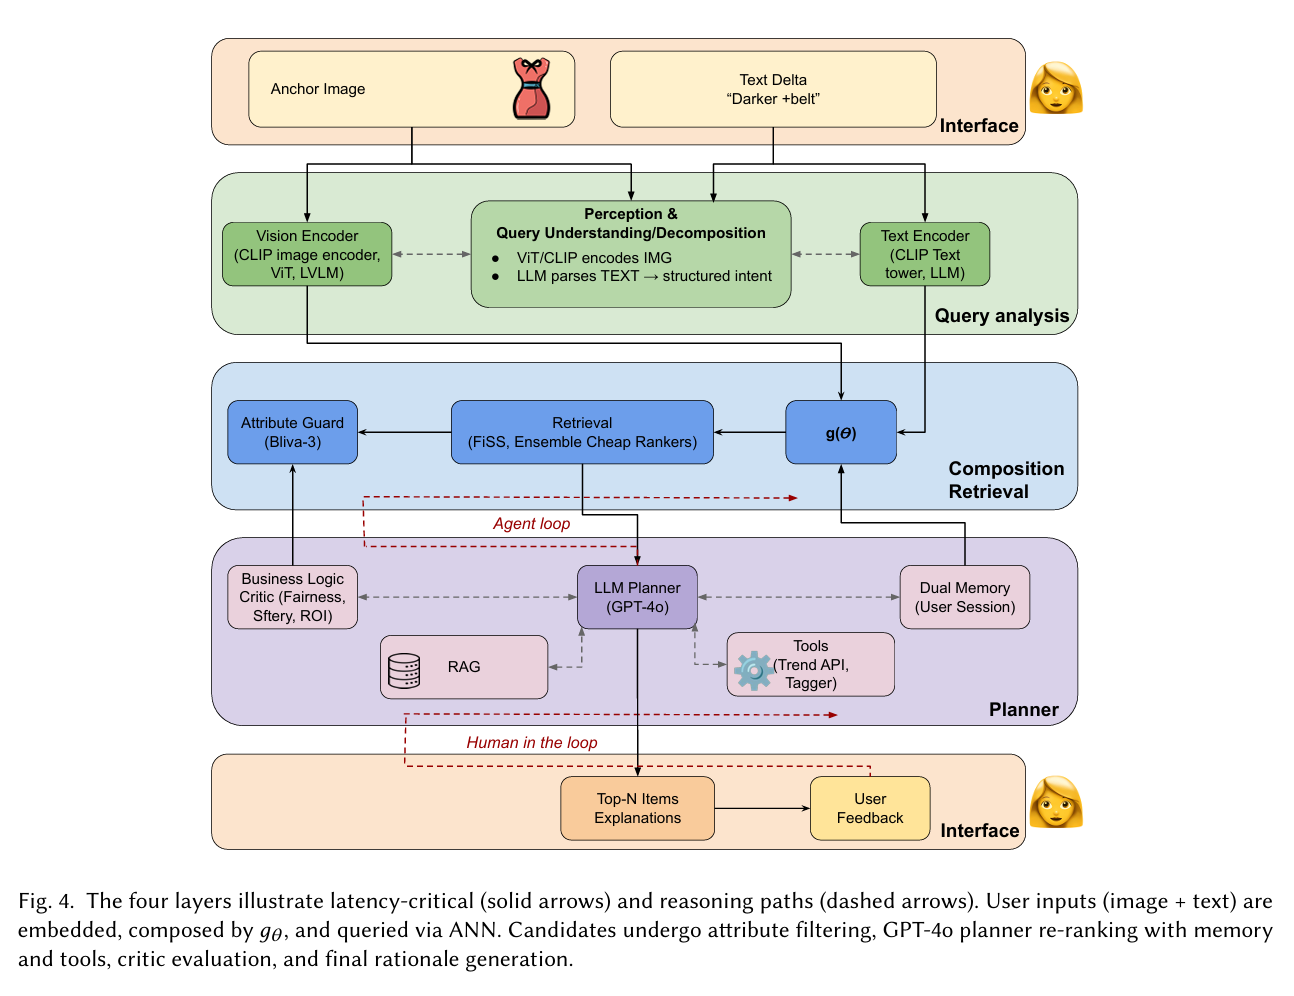
\includegraphics[width=0.9\textwidth]{images/Section3.2/Section3.2.2/LLM_in_outfit_reccomandation.png}
    \caption{Image example of industrial-grade outfit recommendation system.}\citep{deldjoo2025agentic}
    \label{fig:industrial_system}
\end{figure}


This structured reasoning process enables the system to integrate external knowledge, adapt to evolving user intent in real time, and maintain recommendations that remain contextually relevant and aligned with multi-stakeholder objectives \citep{deldjoo2025agentic}.



\subsection{Handling Aesthetic Logic in Outfit Recommendation}
\textbf{\large (1) Add constraint logic to the recommendation pipeline}\\[0.4cm]
This method strengthens professionalism. Constraint logic may be introduced manually, or via training task-specific LLMs to improve recommendation accuracy. However, this will increase development costs and may hinder project progress.

\textbf{\large (2) Directly output via LLM}\\[0.4cm]
Although generally less effective, it significantly reduces implementation time, making it suitable for early development stages while still delivering core functionality.


Therefore, in our project, we will adopt the second approach.




\subsection{Available LLM for Outfit Recommendation}
\begin{table}[H]
\centering
\caption{Comparison of Available LLM Models for Outfit Recommendation}
\label{tab:llm_comparison}
\resizebox{\textwidth}{!}{%
\begin{tabular}{|l|c|c|c|c|}
\hline
\boldmath
\textbf{Model Name} &
\textbf{Release Date} &
\begin{tabular}{@{}c@{}}Specialized in\\Outfit Recommendation\end{tabular} &
\textbf{Fully Functional} &
\begin{tabular}{@{}c@{}}Source Code\\Available\end{tabular} \\
\hline
\unboldmath
\begin{tabular}{@{}c@{}}
Text-Conditioned\\Outfit \\Recommendation
\end{tabular} & 2023 & \CheckedBox & \XBox & \CheckedBox \\
\hline
StePO-Rec & 2024 & \CheckedBox & \CheckedBox & \XBox \\
\hline
CoLLM & 2024 & \XBox & \CheckedBox & \CheckedBox \\
\hline
Gpt-oss & Aug 2025 & \XBox & \CheckedBox & \CheckedBox \\
\hline
\end{tabular}%
}
\end{table}

Based on the studies of \cite{bi2025stepo}, \cite{wang2024text}, \cite{zhang2025collm} and \cite{openai2025gptoss}, Table~\ref{tab:llm_comparison} summarizes the currently available LLMs for outfit recommendation. Existing models exhibit notable shortcomings: task specialization and functional completeness are often mutually exclusive. Systems designed specifically for outfit recommendations usually handle only simple tasks such as filling similar items, while more powerful general-purpose models tend to provide outdated open-source releases. 

Broadening the scope, \textbf{Gpt-oss} can be deployed locally with minimal resource requirements.